\section{Vergleichbare Arbeiten und Produkte}
\label{sec:related-work}

Andere Entwicklungsumgebungen für Datenbanken und auch Generatoren für Abfragemasken gibt es zuhauf. Dieses Kapitel stellt einige der vefügbaren Programme vor, insbesondere im Hinblick auf für diese Arbeit formulierten Prinzipien und unter Betrachtung der avisierten Zielgruppe.

\missing[inline]{Momentan eher eine sehr lose Sammlung denn eine tatsächliche Recherche.}

\subsection{Software: Scratch}

Diese Masterarbeit zieht eine Menge Inspiration aus dem Scratch-Project des Massachusetts Institute of Technology (MIT)\footnote{\url{https://scratch.mit.edu/}}. Bei Scratch handelt es sich um eine Entwicklungsumgebung speziell für Kinder und Jugendliche deren bestimmendes Bedienkonzept Drag \& Drop ist. Scratch lehrt den Umgang mit imperativen und ereignisorientierten Programmierkonzepten und ist damit in Bezug auf die zu vermittelnden Inhalte von dieser Thesis doch deutlich entfernt. Abbildung \ref{fig:scratch-editor-full} zeigt wie die Oberfläche von Scratch für einen Entwickler aussieht, Abbildung \ref{fig:scratch-enduser-full} demonstriert wie sich ein Projekt initial einem Endanwender präsentiert.

Im weiteren Verlauf der Arbeit wird jedoch noch deutlich werden, dass sich esqulino an vielen Stellen dennoch sehr stark an Scratch orientiert. So nutzt auch esqulino einen Drag \& Drop Editor um Syntaxfehler von vornerein auszuschließen und kontextsensitiv mögliche Operationen hervorzuheben. Die Verwendung eines, zu diesem Zeitpunkt allerdings nicht vollständig ausgearbeiteten, Farbkonzeptes nimmt sich ebenfalls Scratch zum Vorbild. Und schließlich ist auch die Zweiteilung eines Projekts in eine Besucheransicht sowie eine Entwickleransicht sowie der fließende Wechsel zwischen diesen Modi eine direkte Inspiration.

Und auch die Wurzeln dieser Arbeit liegen definitiv bei Scratch: Der Arbeitstitel lautete "`Scratch für SQL und Webanwendungen"' und weckt bei Leuten die mit Scratch schon vertraut sind auch die richtigen Assoziationen.

\begin{figure}[p]
  \centering 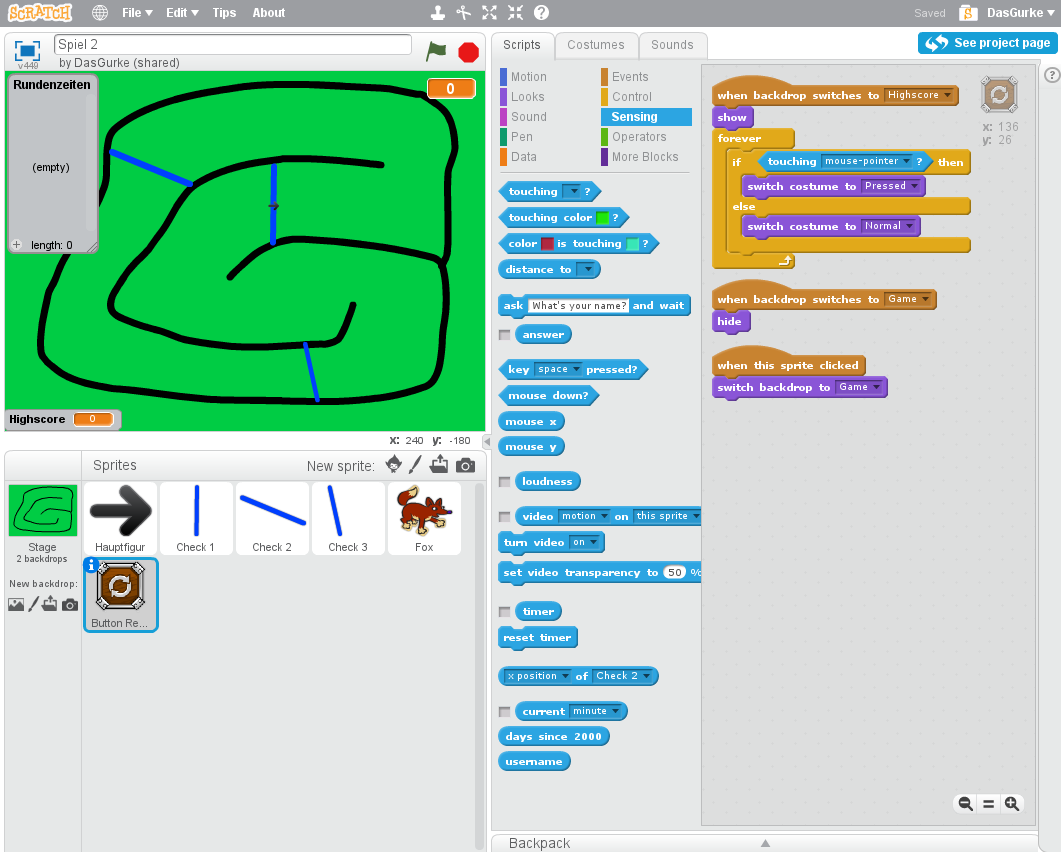
\includegraphics[width=0.7\textwidth]{images/related-work-scratch-editor-full.png}
  \caption{Der Scratch-Editor mit einem Beispielprojekt aus Sicht eines Entwicklers}
  \label{fig:scratch-editor-full}
\end{figure}

\begin{figure}[p]
  \centering 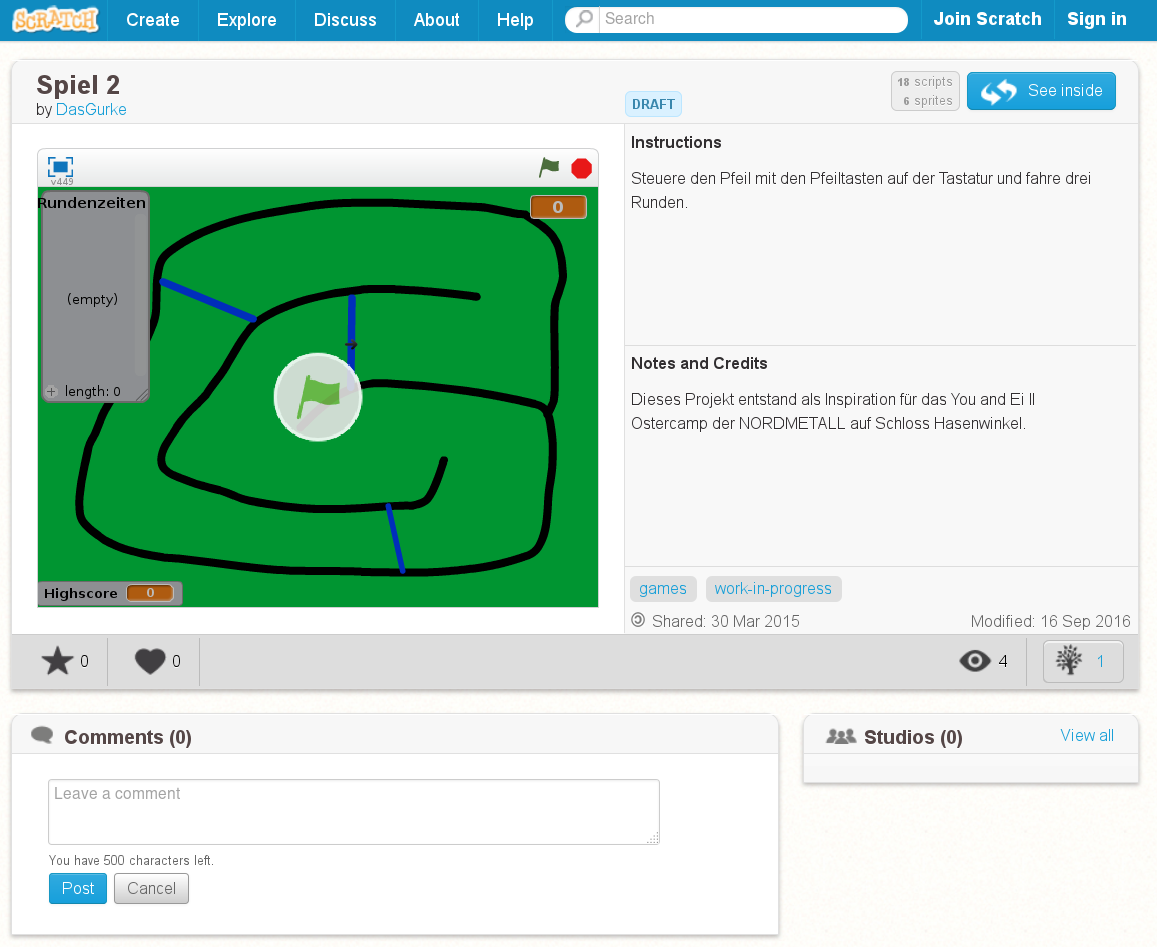
\includegraphics[width=0.7\textwidth]{images/related-work-scratch-project-full.png}
  \caption{Ein Scratch Projekt mit kurzen Handlungsanweisungen und einem Kommentarbereich in der Sicht für Endanwender.}
  \label{fig:scratch-enduser-full}
\end{figure}

\subsection{Software \& Kurs: SqlZoo}

Bei SqlZoo handelt es sich um eines der wenigen Angebote, die SQL-Kenntnisse vermitteln und sich dabei explizit auch an Kinder wenden. Es handelt sich dabei sowohl um einen Kurs in Form einer Sammlung von aufeinander aufbauenden Aufgaben inklusive begleitendem Lehrmaterial als auch eine vergleichsweise rudimentäre, webbasierte Software in welcher die Lernenden ihre ersten Schritte mit SQL machen.

Anders als in Scratch erfolgt die Programmierung der nötigen Abfragen in einem normalen Textfeld, auch Syntax-Hervorhebung ist nicht vorhanden. Die Ergebnisse werden neben dem Textfeld angezeigt und mit dem korrekten Ergebnis verglichen. So können Lernende ihrem Lerntempo gemäß voranschreiten.

\begin{figure}[p]
  \centering \includegraphics[width=\textwidth]{images/related-work-sql-zoo.png}
  \caption{Ergebnisansicht des SqlZoo}
  \label{fig:scratch-enduser-full}
\end{figure}

\subsection{Software \& Kurs: AppCamps}

\info[inline]{Hamburger Start-Up, dass sich mit einer ebenfalls an Scratch orienterten Entwicklungsumgebung Apps für Smartphones entwickeln können.}


\subsection{Software: Visual Studio Lightswitch}

\info[inline]{Generator für Datengetriebene Geschäftsanwendung mit überschaubarer Applikationslogik.}

\subsection{Buch: Die Macht der Abstraktion}

\info[inline]{Buch zum Einstieg in die Programmierung mit einem interessanten, sehr Datentypgetriebenen Ansatz.}

\info[inline]{Die Dr. Scheme Umgebung und auch die verwendete Sprache heißt jetzt ``Racket'' und wird immer noch weiter entwickelt.}

\subsection{Software: Microsoft Access}

\info[inline]{Eher eine Datenbank als eine sinnvolle Eingabemaske für unversierte Benutzer.}

\subsection{Software: MySQL Workbench}

\info[inline]{Wirklich ein Datenbanktool, keinerlei Benutzerschnittstelle für ``normale'' Benutzer.}

%%% Local Variables:
%%% mode: latex
%%% TeX-master: "thesis"
%%% End:
